\documentclass[fontsize=12pt,paper=a4,twoside]{scrartcl}

\newcommand{\grad}{\ensuremath{^{\circ}} }
\renewcommand{\strut}{\vrule width 0pt height5mm depth2mm}

\usepackage[utf8]{inputenc}
\usepackage[final]{pdfpages}
% obere Seitenränder gestalten können
\usepackage{fancyhdr}
\usepackage{moreverb}
% Graphiken als jpg, png etc. einbinden können
\usepackage{graphicx}
%\usepackage{stmaryrd}
% Floats Objekte mit [H] festsetzen
\usepackage{float}
% setzt URLs schön mit \url{http://bla.laber.com/~mypage}
\usepackage{url}
% Externe PDF's einbinden können
\usepackage{pdflscape}
% Verweise innerhalb des Dokuments schick mit " ... auf Seite ... "
% automatisch versehen. Dazu \vref{labelname} benutzen
\usepackage[ngerman]{varioref}
\usepackage[ngerman]{babel}
\usepackage{ngerman}
% Bibliographie
\usepackage{bibgerm}
% Tabellen
\usepackage{tabularx}
\usepackage{supertabular}
\usepackage[colorlinks=true, pdfstartview=FitV, linkcolor=blue,
            citecolor=blue, urlcolor=blue, hyperfigures=true,
            pdftex=true]{hyperref}
\usepackage{bookmark}
\usepackage{enumitem}
\usepackage{color}

\newboolean{langversion} %Deklaration
\setboolean{langversion}{true} %Zuweisung ist 'false' für Blockkurs
\newcommand{\highlight}[1]{\textcolor{blue}{\textbf{#1}}}
\newcommand{\nurlangversion}[0]{%
\ifthenelse{\boolean{langversion}}{\highlight{Muss in SWP-2 ausgefüllt werden}}{\highlight{Entfällt in SWP-1}}}

\newcommand{\swp}[0]{\ifthenelse{\boolean{langversion}}%
{Software--Projekt 2}{Software--Projekt 1}}
\newcommand{\jahr}[0]{2014}
\newcommand{\semester}[0]{\ifthenelse{\boolean{langversion}}{WiSe}{SoSe}}

% Damit Latex nicht zu lange Zeilen produziert:
\sloppy
%Uneinheitlicher unterer Seitenrand:
%\raggedbottom

% Kein Erstzeileneinzug beim Absatzanfang
% Sieht aber nur gut aus, wenn man zwischen Absätzen viel Platz einbaut
\setlength{\parindent}{0ex}

% Abstand zwischen zwei Absätzen
\setlength{\parskip}{1ex}

% Seitenränder für Korrekturen verändern
\addtolength{\evensidemargin}{-1cm}
\addtolength{\oddsidemargin}{1cm}

\bibliographystyle{gerapali}

% Lustige Header auf den Seiten
  \pagestyle{fancy}
  \setlength{\headheight}{70.55003pt}
  \fancyhead{}
  \fancyhead[LO,RE]{\swp\\ \semester{}
  \\Anforderungsspezifikation}
  \fancyhead[LE,RO]{Seite \thepage\\\slshape \leftmark\\\slshape \rightmark}

%Abstände zwischen Tabellenzeilen etwas erhöhen
\renewcommand{\arraystretch}{1.2}

%
% Und jetzt geht das Dokument los....
%

\begin{document}

% Lustige Header nur auf dieser Seite
  \thispagestyle{fancy}
  \fancyhead[LO,RE]{ }
  \fancyhead[LE,RO]{Universität Bremen\\FB 3 -- Informatik\\
  Prof. Dr. Rainer Koschke \\TutorIn: Karsten Hölscher}
  \fancyfoot[C]{}

% Start Titelseite
  \vspace{3cm}

  \begin{minipage}[H]{\textwidth}
  \begin{center}
  \bf
  \Large
  \swp{} \jahr\\
  \smallskip
  \small
  VAK 03-BA-901.02\\
  \vspace{3cm}
  \end{center}
  \end{minipage}
  \begin{minipage}[H]{\textwidth}
  \begin{center}
  \vspace{1cm}
  \bf
  {\Large Anforderungsspezifikation}\\
  \vspace{3ex}
    \begin{figure}[H]
    \centering
    \includegraphics[width=0.25\textwidth]{../woym.png}
    \end{figure}
  \vfill
  \end{center}
  \end{minipage}
  \vfill
  \begin{minipage}[H]{\textwidth}
  \begin{center}
  \sf
  \begin{tabular}{l}
  Tim Hansen \\
  Joshua Hoffmann\\
  Hassan Klait \\
  Adrian Lück \\
  Jurij Schmidt\\
  Falko Schröder
  \end{tabular}
  \\ ~
  \vspace{2cm}
  \\
  \it Version 1.2.3\\ ~
  \end{center}
  \end{minipage}

% Ende Titelseite

% Start Leerseite

\newpage

  \thispagestyle{fancy}
  \fancyhead{}
  \fancyhead[LO,RE]{\swp{}\\ \semester{} \jahr{}
  \\Anforderungsspezifikation}
  \fancyhead[LE,RO]{Seite \thepage\\\slshape \leftmark\\~}
  \fancyfoot{}
  \renewcommand{\headrulewidth}{0.4pt}
  \tableofcontents

\newpage

  \fancyhead[LE,RO]{Seite \thepage\\\slshape \leftmark\\\slshape \rightmark}


%%%%%%%%%%%%%%%%%%%%%%%%%%%%%%%%%%%%%%%%%%%%%%%%%%%%%%%%%%%%%%%%%%%%%%%%
\section*{Version und Änderungsgeschichte}

\begin{tabularx}{\textwidth}{ccX}
Version & Datum & Änderungen \\
\hline
1.0 & 29.10.2014 & Anforderungsspezifikation als \LaTeX Vorlage kopiert. \\
1.1 & 31.10.2014 & Julia Meyer als Persona für Anwendungsfälle hinzugefügt\\ 
1.2 & 01.11.2014 & Auflistung der Verwaltung von Klassen und Personal betreffenden
				   Anwendungsfälle. Detaillierte Beschreibung des Anwendungsfalls \ref{subsubsec:KlasseHinzufuegen} (noch ohne Aktionen).\\
1.2.1 & 02.11.2014 & Kurzbeschreibung der Personal betreffenden Anwendungsfälle. Detaillierte
				   Beschreibung der Anwendungsfälle \ref{subsubsec:KlasseBearbeiten} und \ref{subsubsec:KlasseLoeschen} (noch ohne Aktionen).\\
1.2.2 & 03.11.2014 & Anwendungsfälle \ref{subsubsec:LehrerinHinzufuegen}, \ref{subsubsec:LehrerinBearbeiten}, \ref{subsubsec:LehrerinLoeschen}, \ref{subsubsec:PaedMitarbeiterinHinzufuegen}, \ref{subsubsec:PaedMitarbeiterinBearbeiten} und \ref{subsubsec:PaedMitarbeiterinLoeschen} (noch ohne Aktionen) hinzugefügt.\\
1.2.3 & 04.11.2014 & Klassen und Personal betreffende Aktionen hinzugefügt. Ggf. besteht noch Überarbeitungsbedarf. 
\end{tabularx}


%%%%%%%%%%%%%%%%%%%%%%%%%%%%%%%%%%%%%%%%%%%%%%%%%%%%%%%%%%%%%%%%%%%%%%%%
\section{Einleitung}

\subsection{Vorbemerkung}
Im folgenden wird für Personen des Personals die weibliche Form benutzt, da Frauen an der Grundschule die deutliche Mehrheit bilden. In jedem Fall sind aber auch männliche Lehrer angesprochen.

\subsection{Zweck}
\nurlangversion

  {\em Was ist der Zweck dieser Anforderungsspezifikation? Wer sind
  die LeserInnen?}

\subsection{Rahmen}
\nurlangversion

  {\em Dieser Abschnitt soll einen groben Überblick über die zu
  erstellende Software geben: Welche Produkte sind zu erstellen (mit
  Namen)? Was tut die Software? Auch: Was tut sie nicht? Wozu soll die
  Software verwendet werden?  (Ziele etc.)}

\subsection{Definitionen, Akronyme und Abkürzungen}

\renewcommand{\arraystretch}{2}
\subsubsection{Begriffe aus der Informatik}
\begin{tabular}{p{3cm}p{9.5cm}}
\textbf{Checkbox} & Eine Checkbox ist eine klickbare Box, welche über zwei Zustände verfügt, die sich bei Klick ändern\\
\textbf{GUI} &  Das Graphical User Interface ist die Oberfläche, welche vom Benutzer bedient wird. Der Benutzer bedient lediglich an der GUI. Rechenprozesse o.ä. werden unter der GUI ausgeführt. \\
\textbf{Spinner} & Ein Spinner ist ein Textfeld, in dem man durch klicken von zwei Pfeilen am Textfeld den Inhalt dieses modifiziert.\\
\end{tabular}

\subsubsection{Begriffe aus dem Bereich des Kunden}
\begin{tabular}{p{3cm}p{9.5cm}}
\textbf{Lehrkraft} & Als Lehrkräfte werden Personen angesehen, welche die Bescheinigung haben zu lehren.\\
\textbf{Pädagogische Mitarbeiter} & Als Pädagogische Mitarbeiter werden Personen angesehen, welche sich dem Zweck widmen Kinder zu beaufsichtigen/Aktionen durchführen  und die Lehrkraft aktiv unterstützen, allerdings nicht ohne Beisein einer Lehrkraft Unterricht zu geben.\\
\textbf{Rhythmisierter Unterricht} & Als Rhythmisierten Unterricht bezeichnet man den Wechsel zwischen Lern- und Entspannungsphasen innerhalb eines Unterrichttages. Bspw. auf eine Stunde Mathe folgt eine Stunde Sport.\\
\textbf{Stundenplan} & Ein Stundenplan muss in einer von zwei Ausführungen vorliegen, einerseits ein Lehrerstundenplan und andererseits ein Stundenplan für eine Schulklasse. Aus dem Stundenplan muss ersichtlich sein, wann, wo, mit welchen Materialien, und mit wem sich die betreffende Person aufzuhalten hat.\\
%TODO Falko weitere Anlegen
\end{tabular}

\subsubsection{Definitionen anderweitig verwendeter Begriffe}
\label{subsubsec:anderweitigeBegriffe}
\begin{tabular}{p{3cm}p{9.5cm}}
\textbf{Aktivität} & Eine Aktivität entspricht einer Planungseinheit. Eine Planungseinheit ist ein Tupel der Aspekte Personal Klassen, Stundeninhalte, Räume und Zeiten (Anfang und Ende innerhalb des Zeitrasters). Ein Stundenplan besteht aus einer Menge von Aktivitäten.
\end{tabular}
\renewcommand{\arraystretch}{1.2}

\subsection{Referenzen}

\subsection{Übersicht über das Dokument}
\nurlangversion

  {\em Was enthält die Anforderungsspezifikation? Wie ist das Dokument
  organisiert?}


\section{Allgemeine Beschreibung}
\label{ch:AllgemeineBeschreibung}

\subsection{Ergebnisse der Ist-Analyse}
\nurlangversion

  {\em Hier sollten die Ergebnisse Eurer Ist-Analyse kurz
  zusammengefasst werden. Diese Beschreibung ist hilfreich, um die
  Motivation für die Anforderungen zu verstehen und um sie später
  nachzuvollziehen (z.B.\ dann wenn Anforderungen überarbeitet werden
  sollen, weil sich ihre Rahmenbedingungen geändert haben).
  
  Mögliche Inhalte: 
  \begin{itemize}
    \item Interview/Beobachtung des Kunden oder der Benutzer
    \item Analyse des bisherigen Systems und dessen Probleme 
    \item Analyse ähnlicher Systeme
    \item Auswertung der Benutzerbefragung
    \item Wie sollen die identifizierten Probleme vom neuen System adressiert werden?
  \end{itemize}
  
  N.B.: Dieser Abschnitt ist im IEEE-Standard nicht vorgesehen, aber dennoch
  sinnvoll.}

\subsubsection{Erstes Kundengespräch vom TT.MM.JJJJ}
\nurlangversion

\subsubsection{Interview mit einem Mitarbeiter der ...}
\nurlangversion

{\em Falls durchgeführt}

\subsection{Produktperspektive}

  
\subsubsection{Systemschnittstellen}

  {\em Schnittstellen zu anderen Systemen, z.B.\ Datenimport/-export,
  Konfigurationsdateien, anzubindende externe Dienste und deren Schnittstelle,
  Anbieten der eigenen Funktionalität als API o.ä.}


Das Programm muss mit einer Schnittstelle zu einer leichtgewichtigen Datenbank ausgerüstet werden. Der Transport von Daten findet lediglich innerhalb des Programms und der eingebetteten Datenbank statt.
  

\subsubsection{Benutzerschnittstelle}


  {\em GUI-Design-Richtlinien und Interaktionsmechanismen (nicht
  Screenshots aller Dialoge --- die werden in Kapitel 3 gezeigt --- aber
  evtl.\ ein Screenshot, der einen groben Überblick und Eindruck des
  GUI-Designs gibt).}

%TODO Falko Screenshot einfügen


\subsubsection{Hardwareschnittstellen}


  {\em Schnittstellen zu vorgegebenen Hardwarekomponenten (Name,
  Version).}

Es sind keine Hardwareschnittstellen bekannt.
 

\subsubsection{Softwareschnittstellen}


{\em Softwarebibliotheken und --rahmenwerke (Frameworks), die benutzt
  werden sollen, mit Versionsnummer, Hersteller, Quelle etc. Dazu
  gehört auf jeden Fall Java.}

  \begin{tabular}{|l|l|l|l|}\hline
    \textbf{Name} & \textbf{Version} & \textbf{Hersteller} & \textbf{Quelle} \\\hline
    %TODO Falko Updates und Versionen einfügen
    Java Runtime & 7 Update  & Oracle & \url{http://www.java.com} \\\hline
    JSF Primefaces & 5.1 & PrimeTek &  
   \url{http://www.primefaces.org}\\\hline
    Apache Derby & Derby 10.11.1.1 & Apache & \url{http://www.apache.org} \\\hline
    Spring & & Pivotal Software & \url{http://www.spring.io}\\\hline
  \end{tabular}

\subsubsection{Kommunikationsschnittstellen}
\nurlangversion

{\em Anforderungen an und Bandbreite von Kommunikationsnetzwerken, öffentliche
  oder auch private IP-Adressen?}

Das Programm benötigt keinerlei Kommunikation zu Kommunikationsnetzwerken, lediglich die Verbindung zum lokalen Server.

\subsubsection{Speicherbeschränkung}
\nurlangversion

  {\em min./max.\ verfügbarer Hauptspeicher und Festplattenplatz, knappe Begründung wie Ihr zu
der hier angegebenen Einschätzung gekommen seid}

\subsubsection{Operationen (Betriebsmodi)}

  {\em Welche Betriebsmodi gibt es? Warum? Welche Benutzerklasse darf
  was in welchem Betriebsmodus (Rechte)? Was ist der Zusammenhang
  zwischen Betriebsmodus und Sicherung/Wiederherstellung von Daten?}

Es wird den Betriebsmodus zur Einsicht in erstellte Stundepläne benötigt. Hier wird lediglich Einsicht in den bereits vorhandenen Studenplan gegeben.
Es gibt keine Konfigurationsmöglichkeiten in diesem Modus und daher ist in diesem Modus keine Datensicherung von Nöten.
Jede Benutzergruppe kann diesen Modus ausführen.


Es wird der Bearbeitungsmodus zur Erstellung der verschiedenen Stundenpläne benötigt.
Hier wird der Stundenplan bearbeitet und initial erstellt.
Dieser Modus deckt einen großen Teil des Programms ab und es wird mehrere Konfigurationsmöglichkeiten geben, daher werden in diesem Modus im Hintergrund laufend BackUps erstellt.
Außerdem kann in Schritten zurückgegangen werden, um vorher bestehende Stundenplankonfigurationen wiederaufzurufen.
Es ist also nötig von jedem gemachten Schritt ein BackUp zu erstellen und temporär zu speichern.

Es wird der Konfigurationsmodus zur initialen Einstellung für die Rahmenbedingung des Stundenplans benötigt.
Dieser Modus deckt wichtige Bestandteile der Konfiguration des Stundenplanes ab, welche bei der Erstellung nicht mehr verändert werden können.
Es gilt zu beachten, dass diese Einstellungen erst nach Abfrage geändert werden und dann inital mit Sicherung immer vorliegen, da ohne diese die aktuelle Bearbeitung hinfällig ist und zu Fehlern führen kann.


\subsubsection{Möglichkeiten der lokalen Anpassung}


  {\em Was kann bei Auslieferung des Systems alles konfiguriert
  werden? Z.B. Pfade, Datenbankname, Server-IP usw. Hier ist nicht
  Internationalisierung gemeint!}

Bei der Auslieferung sind grundlegende Funktionen, welche zur Erstellung des Stundenplanes wichtig sind anpassbar.
Weiterhin ist das Verzeichnis, in welchem der Stundenplan schlussendlich gespeichert werden soll anzupassen.


\subsection{Anwendungsfälle}
  
\subsubsection{Verwaltung der Klassen betreffende Anwendungsfälle}

%\paragraph{Mehrere Klassen hinzufügen} Die Anwenderin kann in der Verwaltungs-Ansicht einen Dialog öffnen, um mehrere Klassen hinzuzufügen, sofern noch keine Klassen existieren. Dazu muss lediglich die Anzahl der zu generierenden Klassen für die jeweiligen Jahrgänge angegeben werden. Das System generiert daraus die Klassenbezeichnungen, die aus Jahrgang und Klein- bzw. Großbuchstabe bestehen.

\paragraph{Klasse hinzufügen} Die Anwenderin kann in der Verwaltungs-Ansicht einzelne Klassen hinzufügen. Dazu wählt sie im entsprechenden Dialog den Jahrgang und den Bezeichner in Form eines Klein-/Großbuchstaben aus. Es können auch die Unterrichtsbedarfe der konkreten Klassen angepasst und allgemeine Bemerkungen angegeben werden.

\paragraph{Klasse bearbeiten} Die Anwenderin kann eine bestehende Klasse bearbeiten. Alle Parameter lassen sich ändern.

\paragraph{Klasse löschen} Die Anwenderin kann eine bestehende Klasse löschen.




\subsubsection{Verwaltung des Personals betreffende Anwendungsfälle}

\paragraph{Lehrerin hinzufügen}
Die Anwenderin kann in der Verwaltungsansicht Lehrerinnen hinzufügen. Dazu müssen mindestens Vorname, Nachname, Kürzel und Anzahl der Wochenstunden (in Unterrichtsstunden) angegeben werden. Zusätzlich können Zeitwünsche, Bemerkungen und anrechenbare Ersatzleistungen erfasst werden.

\paragraph{Lehrerin bearbeiten}
Die Anwenderin kann alle Parameter einer bestehenden Lehrerin ändern.

\paragraph{Lehrerin löschen}
Die Anwenderin kann eine vorhandene Lehrerin löschen.

\paragraph{Pädagogische Mitarbeiterin hinzufügen}
Die Anwenderin kann in der Verwaltungsansicht eine pädagogische Mitarbeiterin hinzufügen. Dazu müssen wie bei der Lehrerin mindestens Vorname, Nachname, Kürzel und Anzahl der Wochenstunden in Zeitstunden angegeben werden. Auch hier können zusätzlich Zeitwünsche, Bemerkungen und anrechenbare Ersatzleistungen erfasst werden.

\paragraph{Pädagogische Mitarbeiterin bearbeiten}
Die Anwenderin kann alle Parameter einer bestehenden pädagogischen Mitarbeiterin ändern.

\paragraph{Pädagogische Mitarbeiterin löschen}
Die Anwenderin kann eine bestehende pädagogische Mitarbeiterin löschen.



\subsubsection{Verwaltung der Aktivitätstypen betreffende Anwendungsfälle}

\paragraph{Unterrichtsfach hinzufügen}
Die Anwenderin kann Unterrichtsfächer hinzufügen.

\paragraph{Unterrichtsfach bearbeiten}
Die Anwenderin kann alle Parameter eines bestehenden Unterrichtsfaches ändern.

\paragraph{Unterrichtsfach löschen}
Die Anwenderin kann ein vorhandenes Unterrichtsfach löschen.

\paragraph{Projekt hinzufügen}
Die Anwenderin kann Projekte hinzufügen.

\paragraph{Projekt bearbeiten}
Die Anwenderin kann alle Parameter eines bestehenden Projekts ändern.

\paragraph{Projekt löschen}
Die Anwenderin kann ein vorhandenes Projekt löschen.



\subsubsection{Räume und Standorte betreffende Anwendungsfälle}

\paragraph{Standort hinzufügen}
Die Anwenderin kann einen Standort mit Namen hinzufügen.

\paragraph{Standort löschen}
Die Anwenderin kann einen Standort inklusive aller ihm zugeordneten Räume löschen.

\paragraph{Raum hinzufügen}
Die Anwenderin kann Räume mit ihrer Funktion sowie ihrem tatsächlichen Ort (Raumnummer und Standort) und ähnlichen eindeutigen Ortsbeschreibungen hinzufügen.

\paragraph{Raum bearbeiten}
Die Anwenderin kann einen bestehenden Raum bearbeiten.

\paragraph{Raum löschen}
Die Anwenderin kann einen bestehenden Raum wieder löschen.



\subsubsection{Die Stundenplan-Erstellung betreffende Anwendungsfälle}

\paragraph{Zeitraster für die Planung festlegen}
Die Anwenderin kann zu verplanende Wochentage und deren Beginn und Ende, die übliche Dauer einer Planungseinheit und den zeitlichen Detaillierungsgrad einer Planungseinheit festlegen.  Diese Parameter sind während des Schuljahres veränderbar.

\paragraph{Aktivität hinzufügen}
Die Anwenderin kann einem Stundenplan eine Aktivität (s. \ref{subsubsec:anderweitigeBegriffe}) hinzufügen. Die Aktivität wird auch den Stundenplänen aller anderen Teilnehmer hinzugefügt.

\paragraph{Aktivität bearbeiten}
Die Anwenderin kann eine bestehende Aktivität bearbeiten. \\

\paragraph{Aktivität löschen}
Die Anwenderin kann eine Aktivität löschen. Dabei besteht die Auswahl die Aktivität komplett zu löschen oder nur die Person/Klasse des aktuell betrachteten Stundenplans als Teilnehmer zu entfernen.





\subsubsection{Sonstige Anwendungsfälle}

\paragraph{Backupeinstellungen \"andern}
Die Anwenderin kann die Einstellungen, also die Regelmäßigkeit und den Zeitpunkt, für automatische Backups verändern.

\paragraph{Backup erzeugen}
Die Anwenderin kann manuell ein Backup der Datenbank erzeugen.

\paragraph{Backup wiederherstellen}
Die Anwenderin kann ein Backup wiederherstellen.


\subsection{Charakteristika der Benutzer}

\begin{tabular}{p{3cm}l}
\textbf{Name:} & Julia Meyer \\
\textbf{Alter:} & 36 Jahre\\
\textbf{Tätigkeit:} &  Grundschullehrerin\\
\end{tabular} \\

Frau Meyer ist Grundschullehrerin und unterrichtet hauptsächlich Deutsch, Englisch, Mathe und Musik. Schon früh hat sie sich für diesen Beruf entschieden und auch wenn die Kinder gelegentlich anstrengend sind, hat sie dennoch viel Spaß an ihrer Arbeit.\\
Sie möchte als Hauptverantwortliche die Planung mit der neuen Stundenplansoftware übernehmen, die einige Studierende im Rahmen der Veranstaltung ,,Software-Projekt 2`` für ihre Schule entwickeln sollen, da sie gerne sehen möchte, wie dies von den Studierenden umgesetzt wurde und sie sich erhofft diesen hilfreiches Feedback geben zu können. Nicht zuletzt erhofft sie sich aber auch, dass die neue Software den Planungsprozess deutlich beschleunigt und den Personalbedarf für diesen verringert, so dass sie und ihre Kolleginnen sich stärker auf die Betreuung der Kinder fokussieren können.  \\
Sehr wichtig ist ihr, dass die Software übersichtlich und leicht verständlich ist, denn selbst wenn man wie sie im Umgang mit PCs einigermaßen fit ist, gibt es doch nichts schlimmeres als eine chaotische Software. Da sie in Zukunft hauptverantwortlich für die Planung sein wird, hofft sie auch darauf, dass sie von der Software ausreichend unterstützt wird. Sie wünscht sich z.B. gewarnt zu werden, wenn bei der Planung das Wochenstundenkontingent einer Mitarbeiterin überschritten wird, wenn sie die Zeitwünsche einer Kollegin nicht beachtet hat oder wenn sie versucht eine Kollegin zur selben Zeit für zwei verschiedene Aktivitäten zuzuordnen. \\

\subsection{Einschränkungen}
\label{sec:Einschraenkungen}
{\em Dieser Abschnitt gibt einen groben Überblick über alles, was den
  Entwurf einschränken könnte. Details folgen dann in
  Abschnitt~\ref{ch:DetaillierteBeschreibung} (\glqq Detaillierte
  Beschreibung\grqq). Allgemeine Sicherheitsanforderungen könnten also
  hier kurz beschrieben werden, Details dann im
  Abschnitt~\ref{sec:softwaresystemattribute} zu Systemattributen.

  Beispiele für mögliche Einschränkungen könnten sein (die Liste ist
  nicht vollständig und nicht alle dieser Punkte sind in jedem
  möglichen Projekt relevant):

  \begin{itemize}
   \item feste Vorgaben (z.B. Policies)
   \item gesetzliche Rahmenbedingungen (z.B. Datenschutzaspekte)
   \item Hardwarebeschränkungen
   \item festgelegte Schnittstellen zu anderen Anwendungen
   \item parallele Operationen (z.B. Multithreading)
   \item zu unterstützende Prüffunktionen (auch: Audit-Funktionen;
     z.B. \glqq alle Buchungen im System müssen protokolliert und von
     einem Wirtschaftsprüfer nachvollziehbar sein\grqq)
   \item Steuerungsfunktionen (z.B. \glqq Das System kann von einem
     Techniker von Ferne gewartet werden\grqq)
   \item Anforderungen an die zu verwendende Programmiersprache
   \item Verlässlichkeit; die Verfügbarkeit eines technischen Systems 
       ist die Wahrscheinlichkeit oder das Maß, dass das System 
       bestimmte Anforderungen innerhalb eines vereinbarten
       Zeitrahmens erfüllt. Eine Beispielanforderung könnte sein, dass
       das System an jedem Tag der Woche 24 h lang in Betrieb sein 
       muss und im Jahr höchstens 2 Tage nicht verfügbar sein darf.
   \item Zuverlässigkeit; Software-Zuverlässigkeit wird definiert 
      als die Wahrscheinlichkeit einer fehlerfreien Software-Anwendung 
      über eine spezifizierte Zeitdauer und unter spezifizierten
      Umgebungsbedingungen. Hier könnte zum Beispiel eine zu
      erreichende Testabdeckung in Bezug auf ein Abdeckungsmaß
      gefordert werden: \glqq 90\,\% Anweisungsabdeckung bei den
      Komponententests\grqq.
   \item Kritikalität (Gefährlichkeit eines Versagens) der Anwendung
   \item Sicherheit
  \end{itemize}

}

\subsubsection{Rahmenbedingungen}
\nurlangversion

\subsubsection{Gesetzliche Rahmenbedingungen}
\nurlangversion
 
\subsubsection{Sicherheitskritische Aspekte}
\nurlangversion

\subsection{Annahmen und Abhängigkeiten}
\nurlangversion

  {\em Faktoren, deren Änderung zwangsläufig zu Änderungen an der
  Anforderungsspezifikation führen würde.}



\subsection{Ausblick}
\nurlangversion

  {\em Beschreibt hier knapp, welche Änderungen und Erweiterungen
  zukünftig (d.h.\ nach Auslieferung des Systems) zu erwarten sind.
  Diese Information ist wichtig für den Entwurf, um mögliche
  Änderungen frühzeitig im ersten Entwurf berücksichtigen zu können.
  Der Entwurf kann dann so gestaltet werden, dass die zukünftigen
  Anforderungen leicht realisierbar sind. Die zukünftigen
  Anforderungen sollten realistisch sein, ansonsten könnte ein unnötig
  allgemeiner und damit zu komplizierter Entwurf die Folge sein.  Auch
  dieser Abschnitt ist im IEEE-Standard nicht vorgesehen -- zumindest
  nicht explizit in Form eines eigenständigen Abschnitts. Dennoch
  handelt es sich um wertvolle Information, von der der Entwurf
  profitieren kann.}
  

\section{Detaillierte Beschreibung}
\label{ch:DetaillierteBeschreibung}
{\em Die externen Schnittstellen werden grob in Abschnitt 2
  beschrieben.  Wenn die grobe Beschreibung dort nicht genügt, kann
  sie hier detaillierter ausgeführt werden (wie vom IEEE-Standard
  vorgesehen).}

\subsection{Datenmodell}
  {\em Das Datenmodell im Kontext des Pflichtenhefts ist {\glqq}die
  Darstellung von Informationen und deren Beziehungen in einem
  fachlogischen Konzept{\grqq}. Es soll hier gezeigt werden, welche
  Einheiten für das existierende System relevant sind und welche
  Beziehungen zwischen diesen Einheiten gelten. Es handelt sich
  hierbei noch nicht um ein Datenbankschema oder eine Spezifikation
  von Klassen für die Implementierung (Entwurf), sondern um die
  Modellierung der realen Welt. Das Datenmodell ist leitend für den
  Entwurf (weil alles darin beschrieben sich auch in der Software 
  wiederfinden wird), aber nimmt den Entwurf nicht schon vorweg.
  
  Das Datenmodell soll als UML-Klassendiagramm angegeben werden.
  Wichtig ist hierbei die korrekte Verwendung der UML: Klassen,
  Attribute, Generalisierung, Assoziation, Aggregation, Komposition,
  Multiplizitäten. Außerdem sollte das Diagramm sinnvoll und gut
  lesbar sein. Dazu gehört weiterhin eine kurze Beschreibung des
  Modells mit ergänzenden Informationen, insbesondere wenn die
  Relationen durch ihren Namen nicht selbsterklärend sind. Gebt
  unbedingt ein Mengengerüst für die Daten an: Wie viele Instanzen der
  wichtigsten Klassen werden erwartet? Erwartet Ihr Änderungen im
  Datenvolumen in der Zukunft?}

\begin{figure}[H]
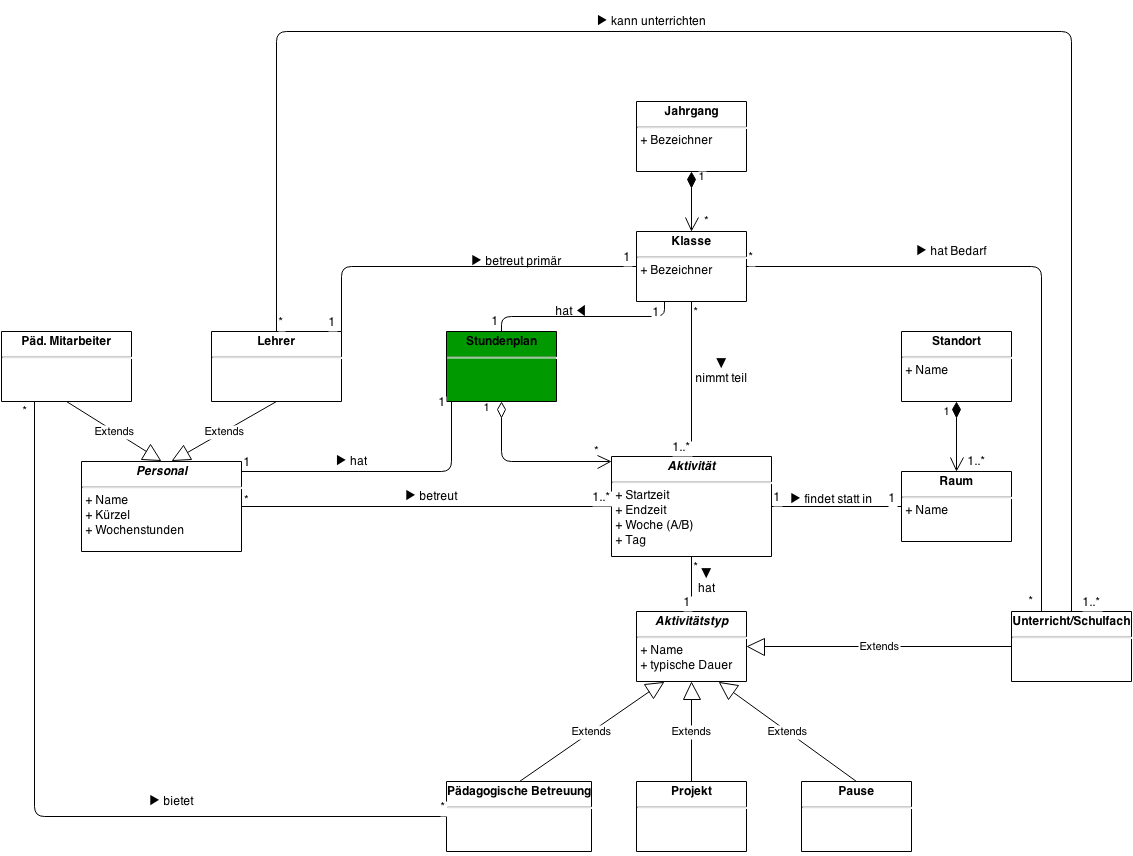
\includegraphics[width=\textwidth]{datenmodell.png}
\end{figure}

\subsection{Anwendungsfälle}

\subsubsection{Anmerkungen zur Notation}
Bei Varianten und Fehler- und Ausnahmefällen dient die numerische Aufzählung auf erster Ebene lediglich der Unterscheidung der Varianten bzw. Fehler- und Ausnahmefällen. Eine numerische Aufzählung auf zweiter oder höherer Ebene beschreibt einen chronologischen Ablauf und eine alphabetische Aufzählung auf zweiter oder höherer Ebene stellt Subvarianten dar.
  
\subsubsection{Abbildungen}

\begin{figure}[H]
\caption{Verwaltungsansicht}
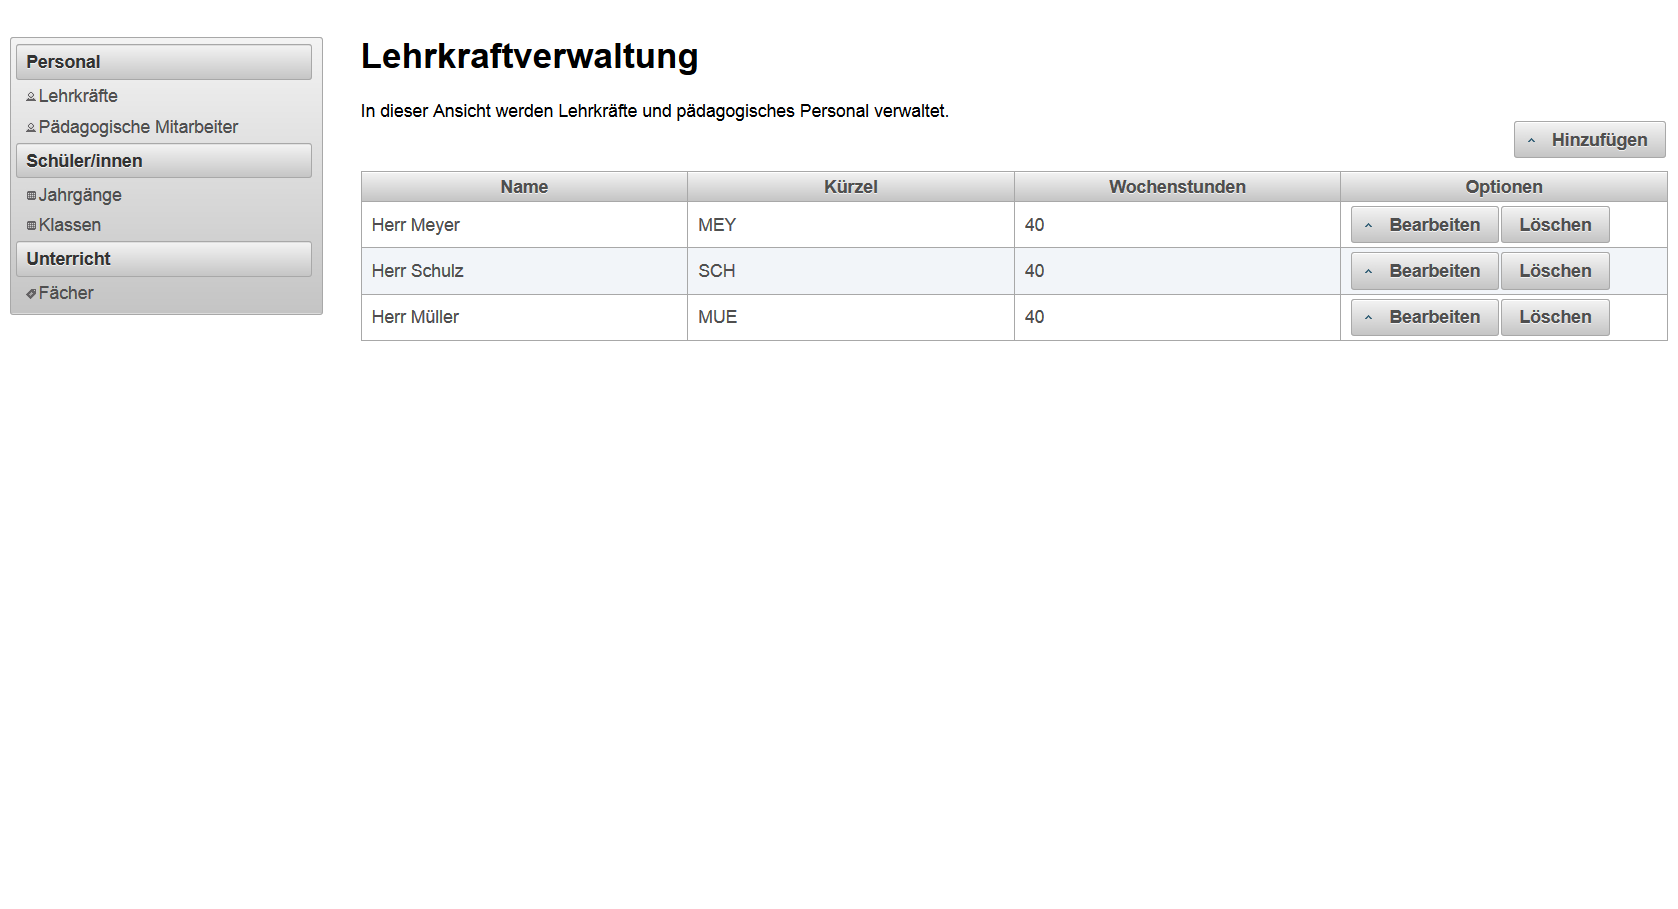
\includegraphics[width=\textwidth]{verwaltungsansicht.png}
\end{figure}
\vspace{5pt}



\subsubsection{Klasse hinzufügen}
\label{subsubsec:KlasseHinzufuegen}
\textbf{Akteurin}
\begin{itemize}
\item Julia Meyer
\end{itemize}
\vspace{5pt}


\textbf{Vorbedingungen}
\begin{enumerate}
\item Die Software wurde von Frau Meyer gestartet und sie befindet sich in der Verwaltungs-Ansicht (s. Abb. 1).
\item Es wurden bereits Schulfächer hinzugefügt.
\item Es sind Unterrichtsbedarfe für die jeweiligen Jahrgänge vorhanden.
\item Es wurden bereits Räume hinzugefügt.
\end{enumerate}
\vspace{5pt}


\textbf{Nichterfüllung von Vorbedingungen}
\begin{itemize}
\item Nichterfüllung von Vorbedingung 2 und 3: Es können keine Unterrichtsbedarfe angegeben werden.
\item Nichterfüllung von Vorbedingung 3: Es können keine dem Jahrgang entsprechenden Unterrichtsbedarfe geladen werden. Eine individuelle Angabe von Unterrichtsbedarfen ist aber möglich, wenn Vorbedingung 2 erfüllt ist.
\item Nichterfüllung von Vorbedingung 4: Es kann kein Klassenraum angegeben werden.
\end{itemize}
\vspace{5pt}

\textbf{Regulärer Ablauf}
\begin{enumerate}
\item Frau Meyer klickt im Navigationsmenü auf der linken Seite auf den Menüpunkt ,,Klassen``.
\item Daraufhin wird im rechten Feld (s. Abb. 1) eine Liste der vorhandenen Klassen angezeigt.
\item Frau Meyer klickt auf den ,,Hinzuf\"ugen``-Button.
\item Es öffnet sich ein modaler ,,Klasse hinzufügen``-Dialog.
\item Frau Meyer wählt in einer Liste den vierten Jahrgang aus. 
\item In einer zweiten Liste werden alle noch verfügbaren Bezeichner für diesen Jahrgang angezeigt.
\item Frau Meyer wählt als Bezeichner ,,A``.
\item Das System lädt die  Unterrichtsbedarfe für den vierten Jahrgang ($\rightarrow$ \texttt{Lade Unterrichtsbedarfe}) und stellt diese im Dialog dar.
\item Frau Meyer möchten den optional anzugebenden Klassenraum auswählen. Sie wählt aus einem Drop-Down-Menü Raum ,,101 (Standort A)`` aus.
\item Frau Meyer möchte die Unterrichtsbedarfe nicht anpassen.
\item Frau Meyer klickt auf den ,,OK``-Button $\rightarrow$ \texttt{Klasse hinzufügen}.
\item Das System erstellt die Klasse. 
\item Das Dialogfenster wird geschlossen.
\end{enumerate}
\vspace{5pt}


\textbf{Varianten}
\begin{enumerate}
\item zu 9: Frau Meyer gibt keinen Klassenraum an (weiter zu 10). 
\item zu 10: Frau Meyer möchte die Unterrichtsbedarfe anpassen.
	\begin{enumerate}[label={\arabic*.}]
	\item Frau Meyer aktiviert die Checkbox ,,Unterrichtsbedarfe anpassen``.
	\item Die Unterrichtsbedarfe sind nun anpassbar.
	\item Frau Meyer ändert in der Auflistung der Schulfächer mit ihren Unterrichtsbedarfen den Bedarf von Deutsch auf 2 Unterrichtsstunden (weiter zu 11).
	\end{enumerate}
\item zu 5-11: Frau Meyer klickt auf den ,,Abbrechen``-Button $\rightarrow$ \texttt{Öffne Abbrechen Bestätigungsdialog}
	\begin{enumerate}[label={\alph*.}]
	\item Frau Meyer bestätigt das Abbrechen (weiter zu 13).
	\item Frau Meyer lehnt das Abbrechen ab (zurück zu 5).
	\end{enumerate}
\end{enumerate}
\vspace{5pt}


\textbf{Nachbedingungen}
\begin{itemize}
\item Nach Ablauf ohne Variante 4a: Die Klasse wurde erfolgreich hinzugefügt.
\item Nach Ablauf mit Variante 4a: Es wurde keine neue Klasse hinzugefügt.
\end{itemize}
\vspace{5pt}


\textbf{Fehler-/Ausnahmefälle}
\begin{enumerate}
\item zu 6: Es sind keine freien Bezeichner mehr vorhanden. 
	\begin{enumerate}[label={\arabic*.}]
	\item Frau Meyer wird mit einem roten Hinweistext auf diesen Umstand hingewiesen (zurück zu 5).
	\end{enumerate}
\item zu Variante 2: Frau Meyer gibt für den Unterrichtsbedarf einen ungültigen Wert an.
		\begin{enumerate}[label={\arabic*.}]
		\item Sie wird umgehend durch ein rotes Highlighting des betreffenden Textfeldes darauf aufmerksam gemacht (zurück zu Variante 2).
		\end{enumerate}
\item zu 8: Es sind keine zu ladenden Unterrichtsbedarfe vorhanden (weiter zu 9).

\end{enumerate}


\subsubsection{Klasse bearbeiten}
\label{subsubsec:KlasseBearbeiten}

\textbf{Akteurin}
\begin{itemize}
\item Julia Meyer
\end{itemize}
\vspace{5pt}


\textbf{Vorbedingungen}
\begin{enumerate}
\item Die Software wurde von Frau Meyer gestartet und sie befindet sich in der Verwaltungs-Ansicht (s. Abb. 1).
\item Es existiert mindestens eine Klasse mit Klassenraum und Unterrichtsbedarfen.
\end{enumerate}
\vspace{5pt}


\textbf{Regulärer Ablauf}
\begin{enumerate}
\item Frau Meyer klickt im Navigationsmenü auf der linken Seite auf den Eintrag ,,Klassen``.
\item Daraufhin wird im rechten Feld (s. Abb. 1) eine Liste der vorhandenen Klassen angezeigt.
\item In der Liste der vorhandenen Klassen f\"uhrt Frau Meyer einen Rechtsklick auf den Eintrag ,,3A`` aus.
\item Es \"offnet sich ein Kontextmen\"u mit den Eintr\"agen ,,Bearbeiten``, ,,L\"oschen`` und ,,Stundenplan anzeigen``.
\item Frau Meyer klickt auf den Eintrag ,,Bearbeiten`` $\rightarrow$\texttt{Öffne ,,Klasse bearbeiten``-Dialog}.
\item Ein ,,Klasse bearbeiten``-Dialog öffnet sich. Alle entsprechenden Felder sind mit den Daten der Klasse gefüllt.
\item Frau Meyer möchte weder den Jahrgang noch den Bezeichner der Klasse ändern.
\item Frau Meyer ändert den Klassenraum auf Raum ,,102 (Standort A)``.
\item Frau Meyer ändert den Unterrichtsbedarf von Mathe auf 2 Unterrichtsstunden.
\item Frau Meyer klickt auf den ,,OK``-Button $\rightarrow$ \texttt{Klasse bearbeiten}.
\item Die Änderungen werden vom System geprüft und übernommen.
\item Das Dialogfenster wird geschlossen.
\end{enumerate}
\vspace{5pt}


\textbf{Varianten}
\begin{enumerate}
\item zu 6: Frau Meyer wählt für den Jahrgang ,,4`` und als Bezeichner ,,A``.
	\begin{enumerate}[label=\arabic*.]
	\item Abweichungen der Unterrichtsbedarfe der vorherigen Klasse ,,3A`` zum vierten Jahrgang werden visualisiert. 
		\begin{enumerate}[label=\alph*.]
		\item Frau Meyer passt die Bedarfe entsprechend an. Falls die Bedarfe im Konflikt mit dem aktuellen Stundenplan der Klasse stehen, wird die Klasse im Warnfenster aufgelistet (weiter zu 7).
		\item Frau Meyer passt die Bedarfe nicht an. Falls die Bedarfe im Konflikt mit dem aktuellen Stundenplan der Klasse stehen, wird die Klasse im Warnfenster aufgelistet (weiter zu 7).
		\end{enumerate}
	\end{enumerate}
\item zu 7: Frau Meyer wählt das leere Feld im Drop-Down-Menü für den Klassenraum (kein Klassenraum).
\item zu 6-9: Frau Meyer klickt auf den ,,Abbrechen``-Button $\rightarrow$ \texttt{Öffne Abbrechen Bestätigungsdialog}
	\begin{enumerate}[label={\alph*.}]
	\item Frau Meyer bestätigt das Abbrechen (weiter zu 11).
	\item Frau Meyer lehnt das Abbrechen ab (zurück zu 6).
	\end{enumerate}
\end{enumerate}
\vspace{5pt}


\textbf{Nachbedingungen}
\begin{itemize}
\item Nach Ablauf ohne Variante 3.1a: Die Klasse wurde im System erfolgreich geändert.
\item Nach Ablauf mit Variante 3.1a: Die Klasse bleibt unverändert.
\end{itemize}
\vspace{5pt}


\textbf{Fehler-/Ausnahmefälle}
\begin{enumerate}
\item zu 5: Beim Laden der Daten tritt ein Fehler auf.
	\begin{enumerate}[label=\arabic*.]
	\item Frau Meyer wird durch einen Hinweis-Dialog darauf hingewiesen, dass sie es erneut versuchen soll und die Klasse ansonsten ggf. löschen muss (zurück zu 4).
	\end{enumerate}
\item zu 8: Frau Meyer gibt für den Unterrichtsbedarf einen ungültigen Wert an.
		\begin{enumerate}[label={\arabic*.}]
		\item Sie wird umgehend durch ein rotes Highlighting des betreffenden Textfeldes darauf aufmerksam gemacht (zurück zu 8).
		\end{enumerate}
\end{enumerate}


\subsubsection{Klasse löschen}
\label{subsubsec:KlasseLoeschen}

\textbf{Akteurin}
\begin{itemize}
\item Julia Meyer
\end{itemize}
\vspace{5pt}


\textbf{Vorbedingungen}
\begin{enumerate}
\item Die Software wurde von Frau Meyer gestartet und sie befindet sich in der Verwaltungs-Ansicht (s. Abb. 1).
\item Es existiert mindestens eine Klasse.
\end{enumerate}
\vspace{5pt}


\textbf{Regulärer Ablauf}
\begin{enumerate}
\item Frau Meyer klickt im Navigationsmenü auf der linken Seite auf den Eintrag ,,Klassen``.
\item Daraufhin wird im rechten Feld (s. Abb. 1) eine Liste der vorhandenen Klassen angezeigt.
\item In der Liste der vorhandenen Klassen f\"uhrt Frau Meyer einen Rechtsklick auf den Eintrag ,,3A`` aus.
\item Es \"offnet sich ein Kontextmen\"u mit den Eintr\"agen ,,Bearbeiten``, ,,L\"oschen`` und ,,Stundenplan anzeigen``.
\item Frau Meyer klickt auf den Eintrag ,,Löschen``.
\item Ein Bestätigungsdialog fordert Frau Meyer auf, das Löschen zu bestätigen.
\item Frau Meyer bestätigt das Löschen $\rightarrow$ \texttt{Klasse(n) löschen}.
\item Der Dialog wird geschlossen.
\item Die Klasse wird gelöscht. Alle Aktivitäten an denen nur diese Klasse beteiligt war, werden ebenfalls gelöscht. Bei allen anderen Aktivitäten an denen diese Klasse teilnahm, wird sie als Teilnehmer entfernt.
\end{enumerate}
\vspace{5pt}


\textbf{Varianten}
\begin{enumerate}
\item zu 7: Frau Meyer lehnt das Löschen ab. 
	\begin{enumerate}[label=\arabic*.]
	\item Der Dialog wird geschlossen, die Klasse bleibt erhalten (Ende des Anwendungsfalls).
	\end{enumerate}
\end{enumerate}
\vspace{5pt}


\textbf{Nachbedingungen}
\begin{itemize}
\item Nach Ablauf mit Variante 1: Alle gewählten Klassen bleiben unverändert.
\item Ansonsten: Die gewählten Klassen inkl. der Aktivitäten an denen keine weitere Klasse mehr teilnehmen würden, werden gelöscht. 
\end{itemize}
\vspace{5pt}

\textbf{Fehler-/Ausnahmefälle}
\begin{enumerate}
\item zu 9: Beim Löschen der Klasse tritt ein Fehler auf.
	\begin{enumerate}[label=\arabic*.]
	\item Frau Meyer wird angemessen auf den Fehler und Behebungsmöglichkeiten hingewiesen (zurück zu 3).
	\end{enumerate}
\end{enumerate}


\subsubsection{Lehrerin hinzufügen}
\label{subsubsec:LehrerinHinzufuegen}
\textbf{Akteurin}
\begin{itemize}
\item Julia Meyer
\end{itemize}
\vspace{5pt}


\textbf{Vorbedingungen}
\begin{enumerate}
\item Die Software wurde von Frau Meyer gestartet und sie befindet sich in der Verwaltungs-Ansicht (s. Abb. 1).
\item Es wurden bereits Schulfächer hinzugefügt.
\item Es wurden bereits Klassen hinzugefügt.
\end{enumerate}
\vspace{5pt}

\textbf{Nichterfüllung von Vorbedingungen}
\begin{itemize}
\item Nichterfüllung von Vorbedingung 2: Es können keine möglichen Stundeninhalte angegeben werden.
\item Nichterfüllung von Vorbedingung 3: Die Lehrerin kann keiner Klasse zugeordnet werden.
\end{itemize}
\vspace{5pt}

\textbf{Regulärer Ablauf}
\begin{enumerate}
\item Frau Meyer klickt im Navigationsmenü auf der linken Seite auf den Eintrag ,,Lehrkr\"afte``.
\item Daraufhin wird im rechten Feld (s. Abb. 1) eine Liste der vorhandenen Lehrer angezeigt.
\item Frau Meyer klickt auf den ,,Hinzufügen``-Button.
\item Ein modaler ,,Lehrerin hinzufügen``-Dialog wird geöffnet.
\item Frau Meyer trägt als Vornamen ,,Julia`` ein.
\item Frau Meyer trägt als Nachnamen ,,Meyer`` ein.
\item Frau Meyer trägt als Kürzel ,,MEY`` ein.
\item Frau Meyer wählt für die Anzahl der Wochenstunden in Unterrichtsstunden mittels des entsprechenden Spinners 28 aus.
\item Frau Meyer ordnet sich den Klassen ,,2A`` und ,,4A`` zu.
\item Frau Meyer wählt aus der Liste der möglichen Stundeninhalte Deutsch, Mathe, Englisch und Musik aus.
\item Frau Meyer klickt auf ,,Anrechenbare Ersatzleistung eintragen``.
\item Es öffnet sich ein weiterer Dialog, in welchem sie die Ersatzleistung eintragen kann.
\item Frau Meyer wählt als anzurechnende Wochenstunden mittels des entsprechenden Spinners 1 aus.
\item Frau Meyer trägt als Bemerkung ,,Pendel`` ein.
\item Frau Meyer klickt auf den ,,OK``-Button des Dialogfensters $\rightarrow$ \texttt{Anrechenbare Ersatzleistung erfassen}.
\item Die anrechenbare Ersatzleistung wird erfasst und das Dialogfenster geschlossen.
\item Frau Meyer möchte keine weiteren anrechenbaren Ersatzleistungen eintragen.
\item Frau Meyer klickt auf den ,,OK``-Button des ,,Lehrerin hinzufügen``-Dialogs $\rightarrow$ \texttt{Lehrerin hinzufügen}.
\item Die Lehrerin wird hinzugefügt.
\item Das Dialogfenster wird geschlossen.
\end{enumerate}
\vspace{5pt}


\textbf{Varianten}
\begin{enumerate}
\item zu 10: Frau Meyer möchte sich dem ganzen dritten Jahrgang zuordnen.
\item zu 11: Frau Meyer möchte keine anrechenbare Ersatzleistung eintragen (weiter zu 18).
\item zu 13-15: Frau Meyer klickt auf den ,,Abbrechen``-Button (weiter zu 16).
\item zu 17: Frau Meyer möchte eine weitere anrechenbare Ersatzleistung eintragen (zurück zu 11).
\item zu 5-11, 17, 18: Frau Meyer klickt auf den ,,Abbrechen``-Button $\rightarrow$ \texttt{Öffne Abbrechen Bestätigungsdialog}.
	\begin{enumerate}[label={\alph*.}]
	\item Frau Meyer bestätigt das Abbrechen (weiter zu 20).
	\item Frau Meyer lehnt das Abbrechen ab (zurück zu 5).
	\end{enumerate}
\end{enumerate}
\vspace{5pt}


\textbf{Nachbedingungen}
\begin{itemize}
\item Nach Ablauf mit Variante 5a: Es wurde keine neue Lehrerin hinzugefügt.
\item Nach Ablauf ohne Variante 5a: Es wurde eine neue Lehrerin hinzugefügt.
\end{itemize}
\vspace{5pt}

\textbf{Fehler-/Ausnahmefälle}
\begin{enumerate}
\item zu 5-7: Frau Meyer gibt in eines der Textfelder einen ungültigen Wert ein, z.B. Zahlen in die Felder für die Namen oder ein schon vorhandenes Kürzel in das Feld für das Kürzel.
	\begin{enumerate}[label=\arabic*.]
	\item Frau Meyer wird umgehend durch ein rotes Highlighting des betreffenden Textfeldes auf den ungültigen Eintrag hingewiesen.
	\end{enumerate}
\end{enumerate}



\subsubsection{Lehrerin bearbeiten}
\label{subsubsec:LehrerinBearbeiten}
\textbf{Akteurin}
\begin{itemize}
\item Julia Meyer
\end{itemize}
\vspace{5pt}


\textbf{Vorbedingungen}
\begin{enumerate}
\item Die Software wurde von Frau Meyer gestartet und sie befindet sich in der Verwaltungs-Ansicht (s. Abb. 1).
\item Es existiert mindestens eine Lehrerin.
\end{enumerate}
\vspace{5pt}


\textbf{Regulärer Ablauf}
\begin{enumerate}
\item Frau Meyer klickt im Navigationsmenü auf der linken Seite auf den Eintrag ,,Lehrkr\"afte``.
\item Daraufhin wird im rechten Feld (s. Abb. 1) eine Liste der vorhandenen Lehrer angezeigt.
\item Frau Meyer f\'uhrt einen Rechtsklick auf den Eintrag ,,Meyer, Julia (MEY)`` aus.
\item Es \"offnet sich ein Kontextmen\"u mit den Eintr\"agen ,,Bearbeiten``, ,,L\"oschen`` und ,,Stundenplan anzeigen``.
\item Frau Meyer klickt auf Eintrag ,,Bearbeiten`` $\rightarrow$ \texttt{Öffne ,,Lehrerin bearbeiten``-Dialog}.
\item Ein modaler ,,Lehrerin bearbeiten``-Dialog öffnet sich. Alle entsprechenden Felder sind mit den Daten der gewählten Lehrerin gefüllt.
\item Frau Meyer möchte den Vornamen nicht ändern.
\item Frau Meyer möchte den Nachnamen nicht ändern.
\item Frau Meyer möchte das Kürzel nicht änden.
\item Frau Meyer ändert die Anzahl der Wochenstunden auf 15.
\item Frau Meyer möchte die betreuten Klassen nicht ändern.
\item Frau Meyer möchte die möglichen Stundeninhalte nicht ändern.
\item Frau Meyer möchte keine anrechenbare Ersatzleistung hinzufügen, ändern oder löschen.
\item Frau Meyer klickt auf den ,,OK```-Button des ,,Lehrerin bearbeiten``-Dialogs $\rightarrow$ \texttt{Lehrerin bearbeiten}.
\item Die Änderungen werden vom System übernommen und der Zeitwunsch endgültig gelöscht.
\item Das Dialogfenster wird geschlossen.
\end{enumerate}
\vspace{5pt}

\textbf{Varianten}
\begin{enumerate}
\item zu 7: Frau Meyer möchte den Vornamen ändern. Sie trägt den neuen Namen in das Vorname-Textfeld ein (weiter zu 8).
\item zu 8: Frau Meyer möchte den Nachnamen ändern. Sie trägt den neuen Namen in das Nachname-Textfeld ein (weiter zu 9).
\item zu 9: Frau Meyer möchte das Kürzel ändern. Sie trägt das neue Kürzel in das Kürzel-Textfeld ein (weiter zu 10).
\item zu 10: Frau Meyer möchte die Anzahl der Wochenstunden nicht ändern (weiter zu 11).
\item zu 11: Frau Meyer möchte die betreuten Klassen ändern. Die Auswahl der neuen Klassen erfolgt
	analog zu Anwendungsfall \ref{subsubsec:LehrerinHinzufuegen}.
\item zu 12: Frau Meyer möchte die möglichen Stundeninhalte ändern. Die Auswahl erfolgt analog zu Anwendungsfall \ref{subsubsec:LehrerinHinzufuegen}.
\item zu 13: Frau Meyer möchte eine anrechenbare Ersatzleistung hinzufügen, ändern oder löschen. Hinzufügen analog zu Anwendungsfall \ref{subsubsec:LehrerinHinzufuegen}. Löschen durch Auswahl der Checkbox hinter dem jeweiligen Eintag.
\item zu 7-14: Frau Meyer klickt auf den ,,Abbrechen``-Button $\rightarrow$ \texttt{Öffne Abbrechen Bestätigungsdialog}.
	\begin{enumerate}[label={\alph*.}]
	\item Frau Meyer bestätigt das Abbrechen (weiter zu 16).
	\item Frau Meyer lehnt das Abbrechen ab (zurück zu 7).
	\end{enumerate}
\end{enumerate}
\vspace{5pt}

\textbf{Nachbedingungen}
\begin{itemize}
\item Nach Ablauf mit Variante 8a: Die gewählte Lehrerin bleibt unverändert.
\item Nach Ablauf ohne Variante 8a: Die Parameter der gewählten Lehrerin wurden entsprechend der gemachten Eingaben geändert.
\end{itemize}
\vspace{5pt}

\textbf{Fehler-/Ausnahmefälle}
\begin{enumerate}
\item zu 10: Die Verringerung der Anzahl der Wochenstunden führt zu einer Überbelastung der Lehrerin. 
	\begin{enumerate}[label=\arabic*.]
	\item Frau Meyer wird entsprechend deutlich auf diesen Umstand hingewiesen.
	\end{enumerate}
\item zu Variante 1-3: Frau Meyer gibt in eines der Textfelder einen ungültigen Wert ein, z.B. Zahlen in die Felder für die Namen oder ein schon vorhandenes Kürzel in das Feld für das Kürzel.
	\begin{enumerate}[label=\arabic*.]
	\item Frau Meyer wird umgehend durch ein rotes Highlighting des betreffenden Textfeldes auf den ungültigen Eintrag hingewiesen.
	\end{enumerate}
\end{enumerate}

\subsubsection{Lehrerin löschen}
\label{subsubsec:LehrerinLoeschen}

\textbf{Akteurin}
\begin{itemize}
\item Julia Meyer
\end{itemize}
\vspace{5pt}

\textbf{Vorbedingungen}
\begin{enumerate}
\item Die Software wurde von Frau Meyer gestartet und sie befindet sich in der Verwaltungs-Ansicht (s. Abb. 1).
\item Es existiert mindestens eine Lehrerin.
\end{enumerate}
\vspace{5pt}

\textbf{Regulärer Ablauf}
\begin{enumerate}
\item Frau Meyer klickt im Navigationsmenü auf der linken Seite auf den Eintrag ,,Lehrkr\"afte``.
\item Daraufhin wird im rechten Feld (s. Abb. 1) eine Liste der vorhandenen Lehrer angezeigt.
\item Frau Meyer f\'uhrt einen Rechtsklick auf den Eintrag ,,Meyer, Julia (MEY)`` aus.
\item Es \"offnet sich ein Kontextmen\"u mit den Eintr\"agen ,,Bearbeiten``, ,,L\"oschen`` und ,,Stundenplan anzeigen``.
\item Frau Meyer klickt auf den Eintrg ,,Löschen``.
\item Ein Bestätigungsdialog fordert Frau Meyer auf, das Löschen zu bestätigen.
\item Frau Meyer bestätigt das Löschen $\rightarrow$ \texttt{Lehrerin löschen}.
\item Der Dialog wird geschlossen.
\item Die gewählte Lehrerin wird gelöscht. Alle Aktivitäten, an denen sonst kein Personal mehr teilnimmt, werden ebenfalls gelöscht, bei allen anderen Aktivitäten wird die gewählte Lehrerin als Teilnehmerin ausgetragen.
\end{enumerate}
\vspace{5pt}

\textbf{Varianten}
\begin{enumerate}
\item zu 7: Frau Meyer lehnt das Löschen ab. 
	\begin{enumerate}[label=\arabic*.]
	\item Der Dialog wird geschlossen, die Lehrerin bleibt erhalten (Ende des Anwendungsfalls).
	\end{enumerate}
\end{enumerate}
\vspace{5pt}

\textbf{Nachbedingungen}
\begin{itemize}
\item Nach Ablauf mit Variante 1: Die Lehrerin wurde nicht gel\"oscht.
\item Ansonsten: Die Lehrerin wurde gel\"oscht. Alle Aktivitäten, an denen sonst kein Personal mehr teilnimmt, wurden ebenfalls gelöscht. Bei allen anderen Aktivitäten wurde die gewählte Lehrerin als Teilnehmerin ausgetragen.
\end{itemize}
\vspace{5pt}

\textbf{Fehler-/Ausnahmefälle}
\begin{enumerate}
\item zu 9: Beim Löschen der Lehrerin tritt ein Fehler auf.
	\begin{enumerate}[label=\arabic*.]
	\item Frau Meyer wird angemessen auf den Fehler und Behebungsmöglichkeiten hingewiesen (zurück zu 4).
	\end{enumerate}
\end{enumerate}

\subsubsection{Pädagogische Mitarbeiterin hinzufügen}
\label{subsubsec:PaedMitarbeiterinHinzufuegen}
Entspricht Anwendungsfall \ref{subsubsec:LehrerinHinzufuegen}, wenn jedes Vorkommnis des Wortes ,,Lehrerin`` durch ,,Pädagogische Mitarbeiterin`` ersetzt wird. Außerdem werden die Wochenstunden in Zeitstunden angegeben und mögliche Stundeninhalte sind keine Schulfächer.


\subsubsection{Pädagogische Mitarbeiterin bearbeiten}
\label{subsubsec:PaedMitarbeiterinBearbeiten}
Entspricht Anwendungsfall \ref{subsubsec:LehrerinBearbeiten} mit in \ref{subsubsec:PaedMitarbeiterinHinzufuegen} genannten Abweichungen. 



\subsubsection{Pädagogische Mitarbeiterin löschen}
\label{subsubsec:PaedMitarbeiterinLoeschen}
Entspricht Anwendungsfall \ref{subsubsec:LehrerinLoeschen}, wenn jedes Vorkommnis des Wortes ,,Lehrerin`` durch ,,Pädagogische Mitarbeiterin`` ersetzt wird. 

\subsubsection{Unterrichtsfach hinzufügen}
%TODO Anwendungsfall schreiben

\subsubsection{Unterrichtsfach bearbeiten}
%TODO Anwendungsfall schreiben

\subsubsection{Unterrichtsfach löschen}
%TODO Anwendungsfall schreiben

\subsubsection{Projekt hinzufügen}
%TODO Anwendungsfall schreiben

\subsubsection{Projekt bearbeiten}
%TODO Anwendungsfall schreiben

\subsubsection{Projekt löschen}
%TODO Anwendungsfall schreiben

\subsubsection{Standort hinzufügen}
\textbf{Akteurin}
\begin{itemize}
\item Julia Meyer
\end{itemize}
\vspace{5pt}

\textbf{Vorbedingungen}
\begin{enumerate}
\item Die Software wurde von Frau Meyer gestartet und sie befindet sich in der Verwaltungs-Ansicht (s. Abb. 1).
\end{enumerate}
\vspace{5pt}

\textbf{Regulärer Ablauf}
\begin{enumerate}
\item Frau Meyer klickt im linken Navigationsmenü auf den Eintrag ,,Standorte und Räume``.
\item Die entsprechende Ansicht wird geöffnet.
\item Frau Meyer möchte einen neuen Standort hinzufügen.
\item Frau Meyer klickt auf den Button ,,Standort hinzufügen``.
\item Ein ,,Standort hinzufügen``-Dialog wird geöffnet.
\item Frau Meyer gibt einen Namen für den Standort ein.
\item Frau Meyer klickt auf den OK-Button $\rightarrow$ \texttt{Standort hinzufügen}.
\item Der Standort wird hinzugefügt.
\end{enumerate}
\vspace{5pt}

\textbf{Varianten}\\
keine
\vspace{5pt}

\textbf{Nachbedingungen}
\begin{itemize}
\item Ein neuer Standort wurde hinzugefügt.
\end{itemize}
\vspace{5pt}

\textbf{Fehler-/Ausnahmefälle}\\
\begin{enumerate}
\item Frau Meyer gibt als Namen einen Namen eines schon existierenden Standortes an.
	\begin{enumerate}[label=\arabic*.]
	\item Sie wird durch ein rotes Highlighting des Textfeldes darauf aufmerksam gemacht, dass dieser Name schon vergeben ist.
	\end{enumerate}
\end{enumerate}

\subsubsection{Standort löschen}
\textbf{Akteurin}
\begin{itemize}
\item Julia Meyer
\end{itemize}
\vspace{5pt}

\textbf{Vorbedingungen}
\begin{enumerate}
\item Die Software wurde von Frau Meyer gestartet und sie befindet sich in der Verwaltungs-Ansicht (s. Abb. 1).
\item Es existiert ein Standort.
\end{enumerate}
\vspace{5pt}

\textbf{Regulärer Ablauf}
\begin{enumerate}
\item Frau Meyer klickt im linken Navigationsmenü auf den Eintrag ,,Standorte und Räume``.
\item Die entsprechende Ansicht wird geöffnet.
\item Frau Meyer wählt mithilfe des Drop-Down-Menüs den zu löschenden Standort.
\item Eine Liste aller Räume, die an diesem Standort liegen, wird angezeigt.
\item Frau Meyer klickt auf den ,,Löschen``-Button.
\item Ein Bestätigungsdialog erscheint und fordert Frau Meyer auf, das Löschen des Standortes inklusive aller dort eingetragenen Räume zu bestätigen.
\item Frau Meyer bestätigt das Löschen $\rightarrow$ \texttt{Standort löschen}.
\item Der Standort und alle dort eingetragenen Räume werden gelöscht.
\end{enumerate}
\vspace{5pt}

\textbf{Varianten}
\begin{enumerate}
\item zu 7: Frau Meyer bestätigt das Löschen nicht (Ende des Anwendungsfalles).
\end{enumerate}
\vspace{5pt}

\textbf{Nachbedingungen}
\begin{itemize}
\item Nach Ablauf mit Variante 1: Weder der Standort noch einer der dort eingetragenen Räume wurde gelöscht.
\item Nach Ablauf ohne Variante 1: Der Standort sowie alle dort eingetragenen Räume wurde gelöscht.
\end{itemize}
\vspace{5pt}

\textbf{Fehler-/Ausnahmefälle}
\begin{enumerate}
\item zu 8: Beim Löschen tritt ein Fehler auf.
	\begin{enumerate}[label=\arabic*.]
	\item Frau Meyer wird durch einen Warndialog auf diesen Umstand hingewiesen.
	\end{enumerate}
\end{enumerate}

\subsubsection{Raum hinzufügen}
\textbf{Akteurin}
\begin{itemize}
\item Julia Meyer
\end{itemize}
\vspace{5pt}

\textbf{Vorbedingungen}
\begin{enumerate}
\item Die Software wurde von Frau Meyer gestartet und sie befindet sich in der Verwaltungs-Ansicht (s. Abb. 1).
\item Es existiert ein Standort.
\end{enumerate}
\vspace{5pt}

\textbf{Regulärer Ablauf}
\begin{enumerate}
\item Frau Meyer klickt im linken Navigationsmenü auf den Eintrag ,,Standorte und Räume``.
\item Die entsprechende Ansicht wird geöffnet.
\item Frau Meyer wählt mithilfe des Drop-Down-Menüs den Standort, für welchen sie einen Raum erstellen möchte.
\item Eine Liste aller Räume, die an diesem Standort liegen, wird angezeigt.
\item Frau Meyer klickt auf den ,,Raum hinzufügen``-Button neben dieser Liste.
\item Ein ,,Raum hinzufügen``-Dialog wird geöffnet.
\item Frau Meyer trägt als Namen/Raumnummer für den Raum ,,101`` ein.
\item Frau Meyer trägt als Funktion ,,Musikzimmer`` ein.
\item Frau Meyer möchte keinen weiteren Standortangaben eintragen.
\item Frau Meyer klickt auf den ,,OK``-Button $\rightarrow$ \texttt{Raum hinzufügen}.
\item Der Raum wird erstellt und in der Liste der zum Standort gehörenden Räume angezeigt.
\item Der Dialog wird geschlossen.
\end{enumerate}
\vspace{5pt}

\textbf{Varianten}
\begin{enumerate}
\item zu 8: Frau Meyer möchte keine Funktion angeben (weiter zu 9).
\item zu 9: Frau Meyer möchte weitere Standortangaben machen. 
	\begin{enumerate}[label=\arabic*.]
	\item Frau Meyer trägt die Angaben in die entsprechende Textarea ein (weiter zu 10).
	\end{enumerate}
\item zu 7-10: Frau Meyer klickt auf den ,,Abbrechen``-Button $\rightarrow$ \texttt{Öffne Abbrechen Bestätigungsdialog}.
	\begin{enumerate}[label={\alph*.}]
	\item Frau Meyer bestätigt das Abbrechen (weiter zu 12).
	\item Frau Meyer lehnt das Abbrechen ab (zurück zu 7).
	\end{enumerate}
\end{enumerate}
\vspace{5pt}

\textbf{Nachbedingungen}
\begin{itemize}
\item Nach Ablauf mit Variante 3a: Es wurde kein neuer Raum hinzugefügt.
\item Nach Ablauf ohne Variante 3a: Es wurde ein neuer Raum hinzugefügt.
\end{itemize}
\vspace{5pt}

\textbf{Fehler-/Ausnahmefälle}
\begin{enumerate}
\item zu 7: Frau Meyer trägt als Namen/Raumnummer einen schon vorhandenen Namen/eine schon vorhandene Raumnummer ein.
	\begin{enumerate}[label=\arabic*.]
	\item Frau Meyer wird durch ein rotes Hightlighting des Textfeldes auf diesen Umstand hingewiesen.
	\end{enumerate}
\end{enumerate}

\subsubsection{Raum bearbeiten}
\textbf{Akteurin}
\begin{itemize}
\item Julia Meyer
\end{itemize}
\vspace{5pt}

\textbf{Vorbedingungen}
\begin{enumerate}
\item Die Software wurde von Frau Meyer gestartet und sie befindet sich in der Verwaltungs-Ansicht (s. Abb. 1).
\item Es existiert ein Standort.
\item Es existiert ein Raum.
\end{enumerate}
\vspace{5pt}

\textbf{Regulärer Ablauf}
\begin{enumerate}
\item Frau Meyer klickt im linken Navigationsmenü auf den Eintrag ,,Standorte und Räume``.
\item Die entsprechende Ansicht wird geöffnet.
\item Frau Meyer wählt mithilfe des Drop-Down-Menüs den Standort, für welchen sie einen Raum bearbeiten möchte.
\item Eine Liste aller Räume, die an diesem Standort liegen, wird angezeigt.
\item Frau Meyer führt einen Rechtsklick auf den Eintrag ,,Raum 101`` aus.
\item Ein Kontext-Menü mit den Einträgen ,,Bearbeiten`` und ,,Löschen`` erscheint.
\item Frau Meyer klickt auf den Eintrag ,,Bearbeiten``.
\item Ein ,,Raum bearbeiten``-Dialog wird geöffnet. Alle Textfelder und ähnlichen Komponenten sind mit den Werten des gewählten Raumes gefüllt.
\item Frau Meyer möchte den Namen bzw. die Raumnummer nicht ändern.
\item Frau Meyer möchte die Funktion nicht ändern.
\item Frau Meyer trägt eine weitere Standortbeschreibung in die entsprechende Textarea ein.
\item Frau Meyer klickt auf den ,,OK``-Button $\rightarrow$ \texttt{Raum bearbeiten}.
\item Der Raum wird geändert.
\item Das Dialogfenster wird geschlossen.
\end{enumerate}
\vspace{5pt}

\textbf{Varianten}
\begin{enumerate}
\item zu 9: Frau Meyer möchte den Namen bzw. die Raumnummer ändern.
	\begin{enumerate}[label={\alph*.}]
	\item Frau Meyer trägt den entsprechenden Namen bzw. die Raumnummer ein (weiter zu 10). 
	\end{enumerate}
\item zu 10: Frau Meyer möchte die Funktion ändern.
	\begin{enumerate}[label={\alph*.}]
	\item Frau Meyer trägt trägt die entsprechende Funktion ein (weiter zu 11). 
	\end{enumerate}
\item zu 9-12: Frau Meyer klickt auf den ,,Abbrechen``-Button $\rightarrow$ \texttt{Öffne Abbrechen Bestätigungsdialog}.
	\begin{enumerate}[label={\alph*.}]
	\item Frau Meyer bestätigt das Abbrechen (weiter zu 14).
	\item Frau Meyer lehnt das Abbrechen ab (zurück zu 9).
	\end{enumerate}
\end{enumerate}
\vspace{5pt}

\textbf{Nachbedingungen}
\begin{itemize}
\item Nach Ablauf mit Variante 1a: Der gewählte Raum wurde nicht geändert.
\item Nach Ablauf ohne Variante 1a: Der gewählte Raum wurde geändert.
\end{itemize}
\vspace{5pt}

\textbf{Fehler-/Ausnahmefälle}
\begin{enumerate}
\item zu 13: Beim Ändern der Parameterwerte des Raumes kommt es zu einem Fehler.
	\begin{enumerate}[label=\arabic*.]
	\item Frau Meyer wird durch einen Warndialog darauf hingewiesen (zurück zu 9).
	\end{enumerate}
\end{enumerate}

\subsubsection{Raum löschen}
\textbf{Akteurin}
\begin{itemize}
\item Julia Meyer
\end{itemize}
\vspace{5pt}

\textbf{Vorbedingungen}
\begin{enumerate}
\item Die Software wurde von Frau Meyer gestartet und sie befindet sich in der Verwaltungs-Ansicht (s. Abb. 1).
\item Es existiert ein Standort.
\item Es existiert ein Raum.
\end{enumerate}
\vspace{5pt}

\textbf{Regulärer Ablauf}
\begin{enumerate}
\item Frau Meyer klickt im linken Navigationsmenü auf den Eintrag ,,Standorte und Räume``.
\item Die entsprechende Ansicht wird geöffnet.
\item Frau Meyer wählt mithilfe des Drop-Down-Menüs den Standort, für welchen sie einen Raum löschen möchte.
\item Eine Liste aller Räume, die an diesem Standort liegen, wird angezeigt.
\item Frau Meyer führt einen Rechtsklick auf den Eintrag ,,Raum 101`` aus.
\item Ein Kontext-Menü mit den Einträgen ,,Bearbeiten`` und ,,Löschen`` erscheint.
\item Frau Meyer klickt auf den Eintrag ,,Löschen``.
\item Ein Bestätigungsdialog fordert zur Bestätigung des Löschens auf.
\item Frau Meyer bestätigt das Löschen $\rightarrow$ \texttt{Raum löschen}.
\item Der gewählte Raum wird gelöscht.
\end{enumerate}
\vspace{5pt}

\textbf{Varianten}
\begin{enumerate}
\item zu 9: Frau Meyer bestätigt das Löschen nicht (Ende des Anwendungsfalls).
\end{enumerate}
\vspace{5pt}

\textbf{Nachbedingungen}
\begin{itemize}
\item Nach Ablauf mit Variante 1: Der gewählte Raum wurde nicht gelöscht.
\item Nach Ablauf ohne Variante 1: Der gewählte Raum wurde gelöscht. Alle Referenzen wurden aufgehoben.
\end{itemize}
\vspace{5pt}

\textbf{Fehler-/Ausnahmefälle}
\begin{enumerate}
\item zu 10: Beim Löschen des Raumes tritt ein Fehler auf.
	\begin{enumerate}[label=\arabic*.]
	\item Frau Meyer wird durch einen Warndialog auf den Fehler hingewiesen.
	\end{enumerate}
\end{enumerate}

\subsubsection{Zeitraster für die Planung festlegen}
%TODO Anwendungsfall schreiben

\subsubsection{Aktivität hinzufügen}
%TODO Anwendungsfall schreiben

\subsubsection{Aktivität bearbeiten}
%TODO Anwendungsfall schreiben

\subsubsection{Aktivität löschen}
%TODO Anwendungsfall schreiben

\subsubsection{Backupeinstellungen ändern}
\textbf{Akteurin}
\begin{itemize}
\item Julia Meyer
\end{itemize}
\vspace{5pt}

\textbf{Vorbedingungen}
\begin{enumerate}
\item Die Software wurde von Frau Meyer gestartet und sie befindet sich in der Verwaltungs-Ansicht (s. Abb. 1).
\end{enumerate}
\vspace{5pt}

\textbf{Regulärer Ablauf}
\begin{enumerate}
\item Frau Meyer klickt im linken Navigationsmenü auf Einstellungen.
\item Die Einstellungsansicht öffnet sich. 
\item Unter dem Eintrag Backups möchte Frau Meyer die Regelmäßigkeit der Backups ändern.
\item Im entsprechenden Drop-Down-Menü hat sie zur Auswahl: täglich, jeden zweiten Tag, jeden vierten Tag, wöchentlich, monatlich und vierteljährlich.
\item Frau Meyer wählt ,,monatlich``.
\item Frau Meyer möchte den Zeitpunkt für die Ausführung des Backups ändern.
\item Frau Meyer wählt den 15. des Monats als Tag für die Ausführung des Backups aus.
\item Frau Meyer wählt 12:00 Uhr als Zeit für die Ausführung des Backups aus.
\item Frau Meyer klickt auf ,,Übernehmen`` $\rightarrow$ \texttt{Backupeinstellungen übernehmen}.
\item Die Einstellungen werden vom System übernommen.
\end{enumerate}
\vspace{5pt}

\textbf{Varianten}
\begin{enumerate}
\item zu 5: Frau Meyer wählt ,,täglich``, ,,jeden zweiten Tag`` oder ,,jeden vierten Tag``.
	\begin{enumerate}[label=\arabic*.]
	\item Frau Meyer kann eine Uhrzeit für die Durchführung des Backups festlegen (weiter zu 8).
	\end{enumerate}
\item 4-9: Frau Meyer schließt das Einstellungsfenster. Die Änderungen werden nicht übernommen (Ende des Anwendungsfalls).
\end{enumerate}
\vspace{5pt}

\textbf{Nachbedingungen}
\begin{itemize}
\item Nach Ausführung ohne Variante 2: Die Backupeinstellungen wurden erfolgreich geändert.
\item Nach Ausführung mit Variante 2: Die Backupeinstellungen wurden nicht geändert.
\end{itemize}
\vspace{5pt}

\textbf{Fehler-/Ausnahmefälle}\\
keine

\subsubsection{Backup erzeugen}
\textbf{Akteurin}
\begin{itemize}
\item Julia Meyer
\end{itemize}
\vspace{5pt}

\textbf{Vorbedingungen}
\begin{enumerate}
\item Die Software wurde von Frau Meyer gestartet und sie befindet sich in der Verwaltungs-Ansicht (s. Abb. 1).
\end{enumerate}
\vspace{5pt}

\textbf{Regulärer Ablauf}
\begin{enumerate}
\item Frau Meyer klickt im linken Navigationsmenü auf Einstellungen.
\item Die Einstellungsansicht öffnet sich. 
\item Unter dem Eintrag Backups klickt Frau Meyer auf den Button ,,Manuelles Backup erzeugen`` $\rightarrow$ \texttt{Backup erzeugen}.
\item Die Datenbank wird so lange eingefroren, bis das Backup erzeugt wurde.
\end{enumerate}
\vspace{5pt}

\textbf{Varianten}\\
keine
\vspace{5pt}

\textbf{Nachbedingungen}
\begin{itemize}
\item Es wurde erfolgreich ein Backup erzeugt.
\end{itemize}
\vspace{5pt}

\textbf{Fehler-/Ausnahmefälle}
\begin{enumerate}
\item zu 4: Beim Erzeugen des Backups tritt ein Fehler auf.
	\begin{enumerate}[label=\arabic*.]
	\item Frau Meyer wird durch einen Warndialog auf diesen Umstand hingewiesen.
	\end{enumerate}
\end{enumerate}

\subsubsection{Backup wiederherstellen}
\textbf{Akteurin}
\begin{itemize}
\item Julia Meyer
\end{itemize}
\vspace{5pt}

\textbf{Vorbedingungen}
\begin{enumerate}
\item Die Software wurde von Frau Meyer gestartet und sie befindet sich in der Verwaltungs-Ansicht (s. Abb. 1).
\end{enumerate}
\vspace{5pt}

\textbf{Regulärer Ablauf}
\begin{enumerate}
\item Frau Meyer klickt im linken Navigationsmenü auf Einstellungen.
\item Die Einstellungsansicht öffnet sich. 
\item Unter dem Eintrag Backups befindet sich eine Liste aller vorhandenen Backups.
\item Frau Meyer wählt das wiederherzustellende Backup aus.
\item Frau Meyer klickt auf den Button ,,Backup wiederherstellen``.
\item Ein Dialog der auf die Folgen der Wiederherstellung hinweist, bittet Frau Meyer um Bestätigung für die Wiederherstellung.
\item Frau Meyer bestätigt die Wiederherstellung $\rightarrow$ \texttt{Backup wiederherstellen}.
\item Es wird ein Backup des aktuellen Datenbankzustandes ausgeführt. Anschließend wird das gewählte Backup wiederhergestellt.
\end{enumerate}
\vspace{5pt}

\textbf{Varianten}
\begin{enumerate}
\item zu 7: Frau Meyer bestätigt die Wiederherstellung nicht (Ende des Anwendungsfalls).
\end{enumerate}
\vspace{5pt}

\textbf{Nachbedingungen}
\begin{itemize}
\item Nach Ablauf mit Variante 1: Es wurde kein Backup wiederhergestellt.
\item Nach Ablauf ohne Variante 1: Das ausgewählte Backup wurde wiederhergestellt.
\end{itemize}
\vspace{5pt}

\textbf{Fehler-/Ausnahmefälle}
\begin{enumerate}
\item zu 8: Beim Erzeugen oder Wiederherstellen des Backups tritt ein Fehler auf.
	\begin{enumerate}[label=\arabic*.]
	\item Frau Meyer wird durch einen Warndialog auf diesen Umstand hingewiesen.
	\end{enumerate}
\end{enumerate}


\subsection{Aktionen}

\subsubsection{Verwaltung der Klassen betreffende Aktionen}

\paragraph{Lade Unterrichtsbedarfe}\mbox{}\\

\begin{tabularx}{\textwidth}{p{4cm}X}
Parameter & \begin{itemize}[itemsep=0pt, leftmargin = 0.5cm]
			\item \texttt{Klasse}
			\end{itemize}\\
Aktion & Lädt die Unterrichtsbedarfe der übergebenen Klasse. Hat die spezifische Klasse keine eigenen definierten Unterrichtsbedarfe, werden die vom entsprechenden Jahrgang geladen.\\
Max. Ausführungszeit & 1 Sek. 
\end{tabularx}\\


\paragraph{Klasse hinzufügen}\mbox{}\\

\begin{tabularx}{\textwidth}{p{4cm}X}
Parameter & \begin{itemize}[itemsep=0pt, leftmargin = 0.5cm]
			\item \texttt{Jahrgang}
			\item \texttt{Bezeichner}
			\item \texttt{Raum}
			\item \texttt{Unterrichtsbedarfe}
			\end{itemize}\\
Aktion & Erzeugt eine neue Schulklasse mit den übergebenen Parameterwerten. Raum und Unterrichtsbedarfe sind optional. Wird kein Raum übergeben, hat die Klasse keinen zugeordneten Klassenraum, werden keine Unterrichtsbedarfe übergeben, werden die jahrgangsweiten verwendet.\\
Max. Ausführungszeit & 1 Sek. 
\end{tabularx}\\


\paragraph{Öffne ,,Klasse bearbeiten``-Dialog}\mbox{}\\

\begin{tabularx}{\textwidth}{p{4cm}X}
Parameter & \begin{itemize}[itemsep=0pt, leftmargin = 0.5cm]
			\item \texttt{Klasse}
			\end{itemize}\\
Aktion & Ein ,,Klasse bearbeiten``-Dialog wird erzeugt, für die entsprechenden Textfelder und anderen GUI-Elemente werden die Parameterwerte der übergebenen Klasse geladen. Der Dialog wird dem Benutzer dann angezeigt.\\
Max. Ausführungszeit & 1 Sek. 
\end{tabularx}\\


\paragraph{Klasse bearbeiten}\mbox{}\\

\begin{tabularx}{\textwidth}{p{4cm}X}
Parameter & \begin{itemize}[itemsep=0pt, leftmargin = 0.5cm]
			\item \texttt{Klasse}: Die zu bearbeitende Klasse.
			\item \texttt{Jahrgang}: Der neue Jahrgang.
			\item \texttt{Bezeichner}: Der neue Bezeichner.
			\item \texttt{Raum}: Der neue Raum.
			\item \texttt{Unterrichtsbedarfe}: Die neuen Unterrichtsbedarfe.
			\end{itemize}\\
Aktion & Die zu bearbeitende Klasse wird entsprechend der übergebenen Parameterwerte angepasst. \\
Max. Ausführungszeit & 1 Sek. 
\end{tabularx}\\


\paragraph{Klasse löschen}\mbox{}\\

\begin{tabularx}{\textwidth}{p{4cm}X}
Parameter & \begin{itemize}[itemsep=0pt, leftmargin = 0.5cm]
			\item \texttt{Klasse}
			\end{itemize}\\
Aktion & Es werden alle Aktivitäten der zu löschenden Klasse durchgegangen. Bei allen Aktivitäten, wo das Entfernen der Klasse als Teilnehmer zur Folge hätte, dass keine Klasse mehr an der Aktivität teilnehmen würde, wird die gesamte Aktivität aus dem System und der Datenbank gelöscht. Bei allen anderen Aktivitäten wird die Klasse als Teilnehmer entfernt und die Aktivitäten in der Datenbank aktualisiert. Alle weiteren Referenzen  auf die zu löschende Klasse (etwa bei einem Lehrer, der diese Klasse primär betreut) werden aufgelöst. \\
Max. Ausführungszeit & 3 Sek. 
\end{tabularx}\\


\subsubsection{Verwaltung des Personals betreffende Aktionen}

Die im folgenden aufgeführten Aktionen gelten mit der Abweichung, dass Stundeninhalt für päd. Personal (ohne teilnehmenden Lehrer an einer Aktivität) keine Schulfächer sind. Ansonsten muss in der Regel nur das Wort ,,Lehrerin`` durch pädagogische Mitarbeiterin ersetzt werden.\\

\paragraph{Anrechenbare Ersatzleistung erfassen}\mbox{}\\

\begin{tabularx}{\textwidth}{p{4cm}X}
Parameter & \begin{itemize}[itemsep=0pt, leftmargin = 0.5cm]
			\item \texttt{Wochenstunden}: Die anzurechnenden Wochenstunden.
			\item \texttt{Bemerkung}: Eine Bemerkung zu der anzurechnenden Ersatzleistung.
			\end{itemize}\\
Aktion & Die Anzahl der Wochenstunden werden zusammen mit der Bemerkung  zwischengespeichert.\\
Max. Ausführungszeit & 0,1 Sek. 
\end{tabularx}

\clearpage
\paragraph{Lehrerin hinzufügen}\mbox{}\\

\hypertarget{par:LehrerinHinzufuegen}{
\begin{tabularx}{\textwidth}{p{4cm}X}
Parameter & \begin{itemize}[itemsep=0pt, leftmargin = 0.5cm]
			\item \texttt{Vorname}
			\item \texttt{Nachname}
			\item \texttt{Kürzel}
			\item \texttt{Wochenstunden} (in Unterrichtsstunden)
			\item \texttt{Liste von Klassen}: Optional. Primär betreute Klassen, der zu erstellenden Lehrerin.
			\item \texttt{Liste von Jahrgängen}: Optional. Primär betreute Jahrgänge, der zu erstellenden Lehrerin.
			\item \texttt{Liste von anrechenbaren Ersatzleistungen}: Optional.
			\item \texttt{Liste von möglichen Stundeninhalten}: Optional. Schulfächer und Projekte.
			\end{itemize}\\
Aktion &  So lange mindestens Vorname, Nachname, Kürzel und Wochenstunden gültige Werte besitzen, kann eine Lehrerin erzeugt und der Datenbank hinzugefügt werden. Gültige Werte sind ungleich \textbf{null}. Für Vorname und Nachname sind eine Folge von Buchstaben und ggf. enthaltene Bindestriche gültig und für die Wochenstunden eine natürliche Zahl. Das Kürzel sollte ungleich allen vorhandenen Kürzeln sein.  Bei ungültigen Werten wird ein Fehler geworfen. Alle anderen Parameter sind optional. Es wird geprüft, ob die Liste der anrechenbaren Ersatzleistungen möglicherweise im Konflikt mit der Wochenstundenzahl steht, indem sie diese auf 0 oder kleinere Werte verringert. In diesem Fall wird ein Fehler geworfen.  \\
Max. Ausführungszeit & 1 Sek. 
\end{tabularx}}\\


\paragraph{Öffne ,,Lehrerin bearbeiten``-Dialog}\mbox{}\\

\begin{tabularx}{\textwidth}{p{4cm}X}
Parameter & \begin{itemize}[itemsep=0pt, leftmargin = 0.5cm]
			\item \texttt{Lehrerin}
			\end{itemize}\\
Aktion & Ein ,,Lehrerin bearbeiten``-Dialog wird erzeugt, für die entsprechenden Textfelder und anderen GUI-Elemente werden die Parameterwerte der übergebenen Lehrerin geladen. Der Dialog wird dem Benutzer dann angezeigt.\\
Max. Ausführungszeit & 1 Sek.
\end{tabularx}\\

\paragraph{Lehrerin bearbeiten}\mbox{}\\

\begin{tabularx}{\textwidth}{p{4cm}X}
Parameter & \begin{itemize}[itemsep=0pt, leftmargin = 0.5cm]
			\item \texttt{Lehrerin}
			\item \texttt{Vorname}
			\item \texttt{Nachname}
			\item \texttt{Kürzel}
			\item \texttt{Wochenstunden} (in Unterrichtsstunden)
			\item \texttt{Liste von Klassen}: Optional. 
			\item \texttt{Liste von Jahrgängen}: Optional. 
			\item \texttt{Liste von anrechenbaren Ersatzleistungen}: Optional.
			\item \texttt{Liste von möglichen Stundeninhalten}: Optional. Schulfächer und Projekte.
			\end{itemize}\\
Aktion & Diese Aktion ist im Grunde analog zur Aktion \hyperlink{par:LehrerinHinzufuegen}{Lehrerin hinzufügen}, hier wird lediglich eine Lehrerin übergeben für die neue Parameterwerte gesetzt werden sollen. Das übergebene Kürzel darf hier gleich dem der übergebenen Lehrerin sein.\\
Max. Ausführungszeit & 1 Sek.
\end{tabularx}\\

\paragraph{Lehrerin löschen}\mbox{}\\

\begin{tabularx}{\textwidth}{p{4cm}X}
Parameter & \begin{itemize}[itemsep=0pt, leftmargin = 0.5cm]
			\item \texttt{Liste von Lehrerinnen}: Liste der zu löschenden Lehrerinnen. Diese kann auch leer sein oder nur ein Element enthalten.
			\end{itemize}\\
Aktion & Ist die Liste von Lehrerinnen leer, geschieht nichts. Ansonsten werden alle Lehrerinnen der Liste einzeln abgearbeitet. Es werden alle Aktivitäten einer jeden Lehrerin durchgegangen. Bei allen Aktivitäten, wo das Entfernen der entsprechenden Lehrerin zur Folge hätte, dass keine Lehrerin mehr an der Aktivität teilnehmen würde, wird die gesamte Aktivität aus dem System und der Datenbank gelöscht. Bei allen anderen Aktivitäten wird die Lehrerin als Teilnehmerin entfernt und die Aktivitäten in der Datenbank aktualisiert. \\
Max. Ausführungszeit & 3 Sek. 
\end{tabularx}\\


\subsubsection{Verwaltung der Aktivitätstypen betreffende Aktionen}
%TODO Aktionen schreiben



\subsubsection{Räume und Standorte betreffende Aktionen}

\paragraph{Standort hinzufügen}\mbox{}\\
%TODO Aktion schreiben

\paragraph{Standort löschen}\mbox{}\\
%TODO Aktion schreiben

\paragraph{Raum hinzufügen}\mbox{}\\
%TODO Aktion schreiben

\paragraph{Raum bearbeiten}\mbox{}\\
%TODO Aktion schreiben

\paragraph{Raum löschen}\mbox{}\\
%TODO Aktion schreiben

\subsubsection{Die Stundenplan-Erstellung betreffende Aktionen}
%TODO Aktionen schreiben

\subsubsection{Sonstige Aktionen}

\paragraph{Backupeinstellungen übernehmen}\mbox{}\\

\begin{tabularx}{\textwidth}{p{4cm}X}
Parameter & \begin{itemize}[itemsep=0pt, leftmargin = 0.5cm]
			\item \texttt{Regelmäßigkeit}
			\item \texttt{Zeitpunkt}
			\end{itemize}\\
Aktion & Die übergebenen Backupeinstellungen werden direkt im System gesetzt und in die entsprechende Konfigurationsdatei geschrieben. \\
Max. Ausführungszeit & 0,1 Sek. 
\end{tabularx}\\



\paragraph{Backup erstellen}\mbox{}\\

\begin{tabularx}{\textwidth}{p{4cm}X}
Parameter & keine\\
Aktion & Die Datenbank wird eingefroren und als Backup in den entsprechenden Backup-Ordner kopiert. Anschließend wird sie wieder aufgetaut, so dass wieder Einträge geschrieben werden können. \\
Max. Ausführungszeit & je nach Größe der Datenbank, max. 10 Minuten 
\end{tabularx}\\



\paragraph{Backup wiederherstellen}\mbox{}\\

\begin{tabularx}{\textwidth}{p{4cm}X}
Parameter & \begin{itemize}
			\item \texttt{Pfad}: Pfad zum wiederherzustellenden Backup
			\end{itemize}\\
Aktion & Handelt es sich bei dem angegebenen Pfad um einen gültigen Pfad zu einem Backup, wird dieses Backup wiederhergestellt, ansonsten wird ein Fehler geworfen. Bei der Wiederherstellung eines Backups werden auch alle aktuell im System vorhandenen verwaltbaren Objekte (Personal, Klassen, Aktivitätstypen, Aktivitäten, Räume, Standorte, etc.) aufgelöst und durch die wiederhergestellten ausgetauscht.\\
Max. Ausführungszeit & je nach Größe der Datenbank, max. 10 Minuten 
\end{tabularx}\\

%TODO Aktionen schreiben

\subsubsection{Systemweite Aktionen}

\paragraph{Öffne Abbrechen Bestätigungsdialog}\mbox{}\\

\begin{tabularx}{\textwidth}{p{4cm}X}
Parameter & \begin{itemize}[itemsep=0pt, leftmargin = 0.5cm]
			\item \texttt{Quelle}: Das Dialogfenster, zu welchem der Bestätigungsdialog gehört.
			\end{itemize}\\
Aktion & Ein Bestätigungsdialog mit einem Text, der darauf hinweist, dass durch einen Abbruch alle Änderungen verloren gehen wird geöffnet. Bestätigt der Nutzer das Abbrechen, werden der Bestätigungsdialog und das zugehörige Dialogfenster geschlossen. Lehnt der Nutzer das Abbrechen ab, wird lediglich der Bestätigungsdialog geschlossen.\\
Max. Ausführungszeit & 0,5 Sek. 
\end{tabularx}\\
  
  
  
\subsection{Softwaresystemattribute}
\label{sec:softwaresystemattribute}

  {\em Hier werden die sogenannten „nichtfunktionalen Anforderungen“
  spezifiziert. Dazu gehören beispielsweise:
  \begin{itemize}
    \item Performanz
    \item Zuverlässigkeit (Korrektheit, Robustheit, Ausfallsicherheit)
    \item Verfügbarkeit
    \item Sicherheit
    \item Wartbarkeit
    \item Portabilität
  \end{itemize}
}

{\em Die spezifizierten Systemattribute müssen hinreichend konkret und
  überprüfbar formuliert werden.}



\subsection{Weitere Anforderungen}
\nurlangversion

{\em In diesem Abschnitt können weitere relevante Anforderungen
  beschrieben werden, die in keine der oben genannten Abschnitte
  passen.}

\section{Anhang}
\nurlangversion

{\em Hier können weitere detailliertere Ergebnisse aus der Ist-Analyse
  oder andere Informationen, die zur Erstellung der Spezifikation
  gedient haben (z.B. Papierprototypen), angefügt werden.}

\end{document}
